% elemCell.tex      pdflatex ZhCvGo15
% Diffuse globally, compute locally: a cyclist tale
% Tingnan Zhang, Daniel I. Goldman and Predrag Cvitanovi\'c

%\section{Cycles in the elementary cell}
%\label{s-elemCell}

\begin{figure}
  \begin{center}
    (a)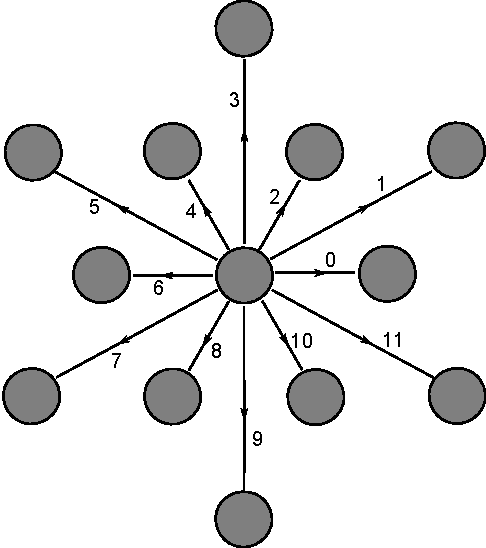
\includegraphics[width=0.27\textwidth]{diffuseDiskDirectionsElCell}
    (b)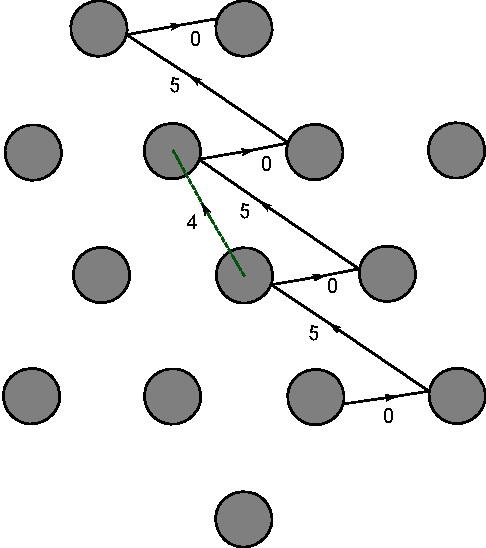
\includegraphics[width=0.27\textwidth]{diffuseDiskDirecsElCell05}
    (c)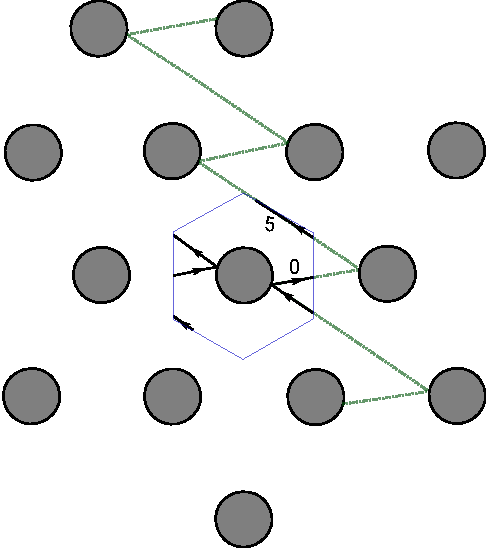
\includegraphics[width=0.27\textwidth]{diffuseDiskDirecsElCell05red}
  \end{center}
  \caption{\label{fig-diskDirectionsElCell}
  Elementary cell symbolic dynamics is obtained by counterclockwise
  labeling the translation vectors connecting the center of the current
  disk to the center of  the next disk. (a) The finite horizon is here
  imposed by limiting jumps from  the center cell to six short jumps
  (even labels $0, 2,\cdots,10$) and six `long' jumps (odd labels $1,
  3,\cdots,11$). (b) Running mode  \cycle{05} advances by $\hn_4$ per
  period. (c) In the elementary cell this is  a \po\ \cycle{05} of
  topological length 2.
  }
\end{figure}

We use the symbolic dynamics developed in \refref{CGS92} and briefly
review the concepts here. With imposed finite horizon there are 12
possible ways of jump from a disk
(\reffig{fig-diskDirectionsElCell}\,(a)). Any trajectory in the full
space can always be constructed from a series of flights, each belongs to
the 12 ``signature jumps''. In particular, a periodic orbit in the
elementary cell is represented as a repeatable string of such symbols.
For example, the bouncing mode between nearest disks is written as
\cycle{06}, meaning that the periodic orbit is consisted of two
successive flights, one traveling towards right (symbol $0$) and the next
reflecting backwards (symbol $6$).

Periodic orbits in the elementary cell can either be stationary in the
full space that goes back to its original place after completing a full
cycle (e.g., \cycle{06} that represents the bouncing of the particle
between two nearest disk); or can be in a running mode that generates a
net displacement along the trajectory (e.g., \cycle{05},
\reffig{fig-diskDirectionsElCell}\,(a) and (c). The stationary cycles
``trap'' the  particle locally for a finite amount of time while the
running cycles advance it. The final diffusion \refeq{eq-ecDiffCoef} can
be conceptually understood as the result of competition between the two
type of cycles.

With the symbolic dynamics, we then use the least action principle to
compute the periodic orbits\rf{DasBuch}. In a planetary Hamiltonian
billiard system, the Maupertuis' principle indicates that the traveling
length along a cycle is minimized. We can solve the problem by optimizing
the total free flight distance with the constraint that links have to
connect the specific disks visited along the orbit.

Elementary cycles found using this method and the corresponding cycle
expansion calculation results are listed in \reftab{TCELL1}. Although the
diffusion coefficient computed using elementary cycles up to $n_p = 8$
matches the numerical experiment value $0.25$, the convergence is not
promising.

\begin{table}[htbp]
%\begin{center}
\begin{tabular}{|r|r|r|l|l|}
\hline
${n_p}$ & \# cycles & $\zeta$(0,0) & $\lambda$ & D \\ \hline\hline
1      & 0      &   -    &   -  &   - \\
2      & 24     & -0.31697 & 1.330 & 0.375\\
3      & 64     & -0.54152 & 1.435 & 0.339\\
4      & 168    & -0.09764 & 1.902 & 0.284\\
5      & 516    &  0.02334 & 2.324 & 0.215\\
6      & 1589   & -0.00481 & 1.975 & 0.133\\
7      & 5700   & -0.01241 & 1.885 & 0.184\\
8      & 20729  & -0.01006 & 1.785 & 0.247\\ \hline

\end{tabular}
\caption{\label{TCELL1}
Cycle expansion results computed Schreiber 1992 calculation\rf{CGS92} (and
  this paper) in elementary cell.
}
\end{table}

For a simple example, see the chain of baker's maps chain of coupled
baker maps studied in \refref{Gaspard92}.

Some confidence can be gained at this point by applying the above
formula~\refeq{TS:formula} to a trivial system, a

In this case there are only four fixed points, all with
stability $\Lambda_p=1/2$, two of
which give rise to the translations $\hn_{p}=\pm 1$.
As the system is
uniformly hyperbolic, all curvature terms are identically zero,
and the fixed points substituted into \refeq{TS:formula} yield
immediately the correct result $D=1/4$.
